Una rete radiomobile permette a terminali radio di utenti (User equipment, UE ) di connettersi a servizi telefonici e/o di dati.
Permette la comunicazione senza interruzioni durante la mobilità.
Le reti radiomobili sono costituite da:
\begin{itemize}
	\item \textbf{Radio Access Network (RAN)}: gestisce la comunicazione via radio con gli UE.
	\item \textbf{Core network (CN)}: interconnette le RAN alle infrastrutture esterne, offre servizi di gestione di connettività e mobilità.
	Si possono ulterioremente distinguere in:
	\begin{itemize}
		\item \textbf{A commutazione di circuito}: permettono l'accesso ai servizi telefonici (2G e 3G).
		\item \textbf{A commutazione di pacchetto}: permettono l'accesso ai servizi di dati (2G, 3G, 4G e 5G)
		e ai servizi telefonici (solo 4G e 5G).
	\end{itemize}
\end{itemize}
\section{Base stations}
L'elemento fondamentale di una RAN è la stazione base (base station, BS), che gestisce la comunicazione radio con gli UE.
Sono quindi collegate alla core network attraverso una rete di backhaul.
\begin{figure}[H]
	\centering
	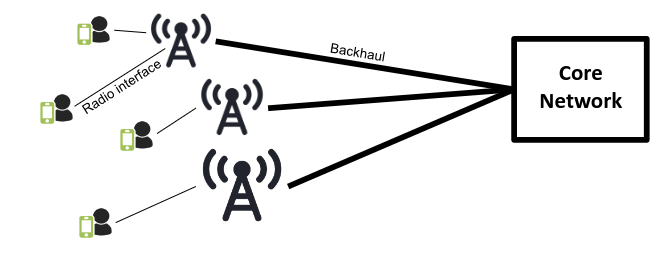
\includegraphics[width=0.8\textwidth]{pictures/8/bs.png}
	\caption{Base station}
\end{figure}
L'area in cui il servizio è offerto viene diviso in celle, ognuna servita da una BS.
Le celle hanno approssimativamente forma esagonale, formando un piastrellamento del piano.
Per poter gestire la mobilità, è necessario permettere quattro procedure:
\begin{itemize}
	\item \textbf{Cell selection}
	\item \textbf{Local update}
	\item \textbf{Paging}
	\item \textbf{Handover}
\end{itemize}
La procedura da scegliere dipende dallo stato del UE, che può essere \textbf{idle} o \textbf{active}.
\subsection{Cell selection}
In mobilità di tipo idle, l'UE seleziona in modo autonomo la BS più conveniente.
Per prima cosa, ascoltano un segnale di beacon che viene trasmesso da tutte le BS a massima potenza, dopodiché scelgono la BS con il segnale più forte.
Generalmente, la potenza del segnale è inversamente proporzionale alla distanza, quindi l'UE sceglie la BS più vicina.
\begin{figure}[H]
	\centering
	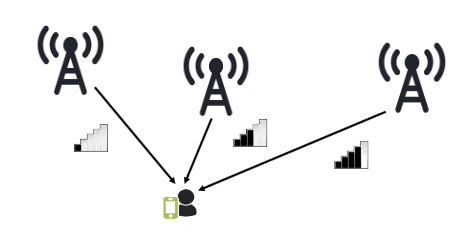
\includegraphics[width=0.6\textwidth]{pictures/8/cellSelection.png}
	\caption{Cell selection}
\end{figure}
\subsection{Location update}
In mobilità di tipo idle, la posizione dell'UE deve essere tracciata a un livello di granularità di \textbf{Location Area (LA)}.
Una location area è un insieme contiguo di celle, identificato da un codice univoco (\textbf{Location Area Identity, LAI}).
La LA corrente di ogni UE è memorizzata in un database, associata all'ID univoco dell'UE.
\begin{figure}[H]
	\centering
	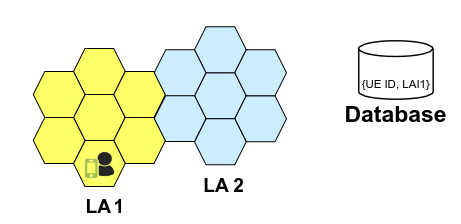
\includegraphics[width=0.6\textwidth]{pictures/8/locationArea.png}
	\caption{Location area}
\end{figure}
Quando un UE si sposta da una LA a un'altra, deve eseguire una procedura di location update,
che consiste nell'inviare un messaggio alla nuova BS, che a sua volta aggiorna il database con la nuova LA dell'UE.
\begin{figure}[H]
	\centering
	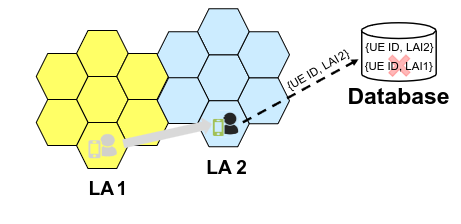
\includegraphics[width=0.6\textwidth]{pictures/8/locationUpdate.png}
	\caption{Location update}
\end{figure}
\subsection{Paging}
Quando una chiamata o un messaggio di dati è destinato a un UE in mobilità di tipo idle, la rete deve localizzarlo per poterlo raggiungere.
Per poterlo fare deve ottenere dal database il LAI del LA corrente e l'ID univoco dell'UE.
Dopodiché, inizia la procedura di paging:
\begin{itemize}
	\item Tutte le BS della LA con il LAI specificato trasmettono in broadcast un messaggio di paging, che include l'ID dell'UE.
	\item L'UE risponde con un messaggio di paging.
	\item La sessione può essere instradata verso la cella corretta, viene cambiato lo stato in attivo.
\end{itemize}
\begin{figure}[H]
	\centering
	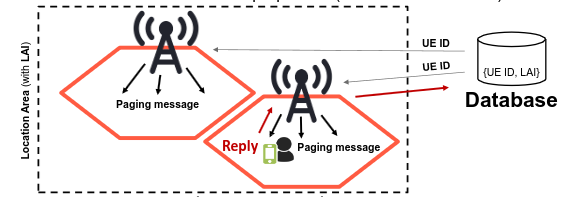
\includegraphics[width=0.6\textwidth]{pictures/8/paging.png}
	\caption{Paging}
\end{figure}
\subsection{Tradeoff paging e location update}
Quando si progetta una rete è necessario chiedersi quale sia la dimensione ottimale delle LA, in termini di celle.
La dimensione delle LA coinvolge due bisogni contrastanti:
\begin{itemize}
	\item \textbf{Pagine più grandi}: più signaling causato dal paging, meno signaling causato dal location update.
	\item \textbf{Pagine più piccole}: meno signaling causato dal paging, più signaling causato dal location update.
\end{itemize}
La dimensione ottimale dipende dalle stime di mobilità degli UE e dalla frequenza con cui ricevono chiamate o messaggi di dati.
\subsection{Handover}
In mobilità di tipo active, la posizione dell'UE è tracciata a livello di cella,
in questo caso la procedura di mobilità è chiamata handover.
Il processo è controllato dalla rete, adatta il routing e impone all'UE di cambiare cella una volta che la nuova connettività è stata configurata (make-before-break).
\begin{figure}[H]
	\centering
	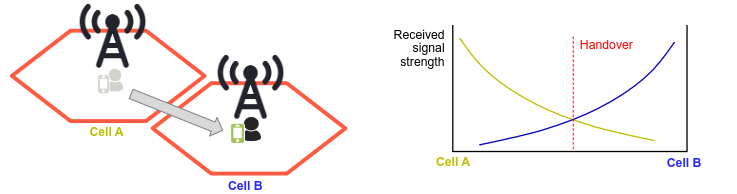
\includegraphics[width=0.6\textwidth]{pictures/8/handover.png}
	\caption{Handover}
\end{figure}
\section{Radio planning}
La posizione e la configurazione delle BS deve esse pianificata, questo processo include due fasi:
\begin{itemize}
	\item \textbf{Pianificazione della copertura}: scelta di dove installare le BS e la loro configurazione.
	\item \textbf{Pianificazione delle frequenze} (o capacity planning): scelta di quali frequenze assegnare a ogni cella, per minimizzare l'interferenza.
\end{itemize}
\begin{figure}[H]
	\centering
	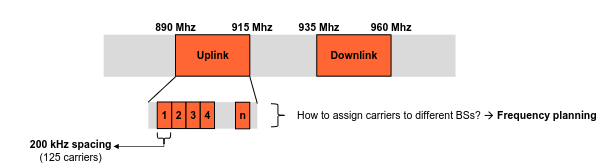
\includegraphics[width=0.8\textwidth]{pictures/8/frequencyPlanning.png}
	\caption{Frequency planning}
\end{figure}
\subsection{Pianificazione della copertura}
Per pianificare la copertura, è necessario considerare quattro fattori correlati:
\begin{itemize}
	\item \textbf{Predizione della propagazione del segnale}
	\item \textbf{Stima del traffico}
	\item \textbf{Posizionamento delle base station}
	\item \textbf{Configurazione delle antenne}
\end{itemize}
\subsubsection{Predizione della propagazione del segnale}
Per pianificare la copertura è importante prevedere la propagazione del segnale,
questo permette di stimare l'area di copertura di una BS.
L'area di copertura è definita come l'area in cui il segnale ricevuto è più forte del segnale proveniente da qualsiasi altra BS.
La forza del segnale dipende dalla potenza emessa, la perdita di propagazione e l'interferenza.
\begin{figure}[H]
	\centering
	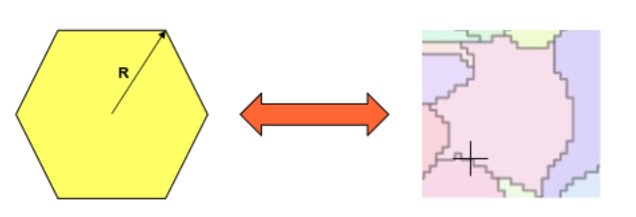
\includegraphics[width=0.6\textwidth]{pictures/8/propagation.png}
	\caption{Signal propagation}
\end{figure}
\subsubsection{Stima del traffico e posizionamento delle BS}
Stimare il traffico che verrà generato in una specifica service area è un compito molto difficile, dipende dalla popolazione, urbanizzazione, presenza del servizio, ecc.
Viene considerato un insieme di posizioni candidate per le BS, basandosi su aspetti tecnici (stima del traffico, morfologia del terreno, ecc.) 
e aspetti non tecnici (inquinamento elettro-magnetico, accordi con i proprietari di immobili, legislazioni locali, ecc.)
\subsubsection{Configurazione delle antenne}
Diversi aspetti vanno considerati, ad esempio:
\begin{itemize}
	\item Diagramma di radiazione
	\item Inclinazione
	\item Massima potenza
	\item Altezza
	\item Capacità della BS
	\item etc.
\end{itemize}
Diverse configurazioni possono essere testate, per esempio con simulazioni, per scegliere quella ottimale.
\bigbreak
Tutti questi aspetti vanno considerati quando bisogna decidere dove posizionare le BS e come configurare le antenne.
Un insieme discreto di \textbf{Test Points (TP)} viene usato per valutare la bontà di una strategia copertura.
Viene utilizzato un modello di ottimizzazione matematica per garantire che ogni TP abbia un livello minimo di copertura, tipicamente minimizzando il costo di installazione.
\begin{figure}[H]
	\centering
	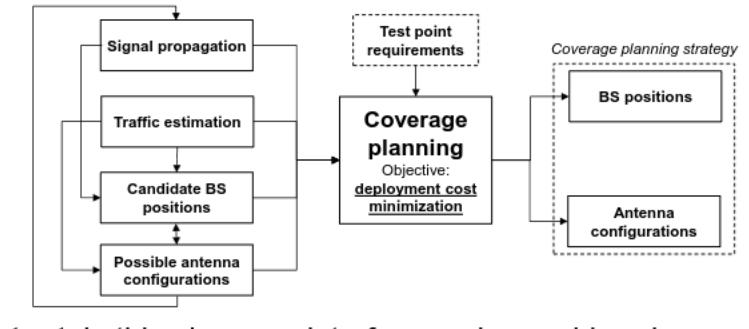
\includegraphics[width=0.8\textwidth]{pictures/8/coveragePlanning.png}
	\caption{Test points}
\end{figure}
\textbf{N.B.}: in questa fase non vengono considerate le interferenze, che invece sono considerate nella fase di pianificazione delle frequenze.
\subsection{Pianificazione delle frequenze}
Nelle vecchie tecnologie (2G) le risorse radio (frequenze) non potevano essere usate tutte da una cella qualsiasi, in quanto avrebbero generato interferenze tra celle adiacenti.
Tuttavia, in qualche modo le frequenze devono essere assegnare a celle diverse, per il principio di reuse, con l'obiettivo di minimizzare l'interferenza.
\break
Data il raggio di propagazione non uniforme, la forma reale di una cella non è esagonale, quest'ultima viene usata solo come approssimazione per determinare il riutilizzo delle frequenze.
\begin{figure}[H]
	\centering
	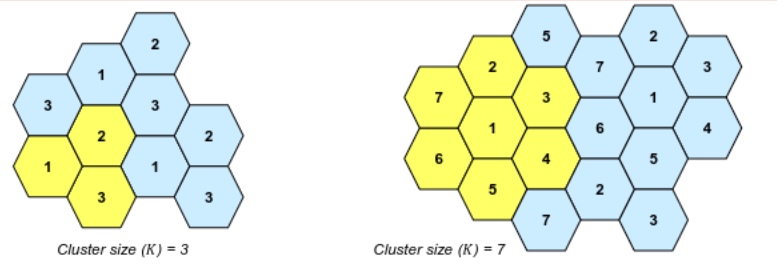
\includegraphics[width=0.8\textwidth]{pictures/8/frequencyReuse.png}
	\caption{Frequency reuse}
\end{figure}
\subsubsection{Cluster}
Per ridurre le interferenze, diverse frequenze vengono assegnate a celle adiacenti, in questo modo si formano dei cluster di celle che usano lo stesso set di frequenze.
Un cluster ampio porta ad avere meno interferenze, ma anche meno capacità per cella.
Solo alcuni valori $K$ (numero di celle per cluster) sono accettabili, ad esempio $K=3,4,7,9$.
Allora l'efficienza di riutilizzo delle frequenze è data da $\frac{1}{K}$, quindi $K$ deve essere scelto in modo da bilanciare interferenza e capacità.
Si può avere dimensioni di cluster uguale a 1 se si utilizzano frequenze ortogonali o codici ortogonali, queste tecniche sono usage in 3G, 4G e 5G rendendo inutile la pianificazione delle frequenze.
Data la forma esagonale delle celle, le forme valide dei cluster sono quelle che risultano, per una cella specifica nel cluster, nelle sei celle più vicine che usano la stessa frequenza alla stessa distanza.
\begin{figure}[H]
	\centering
	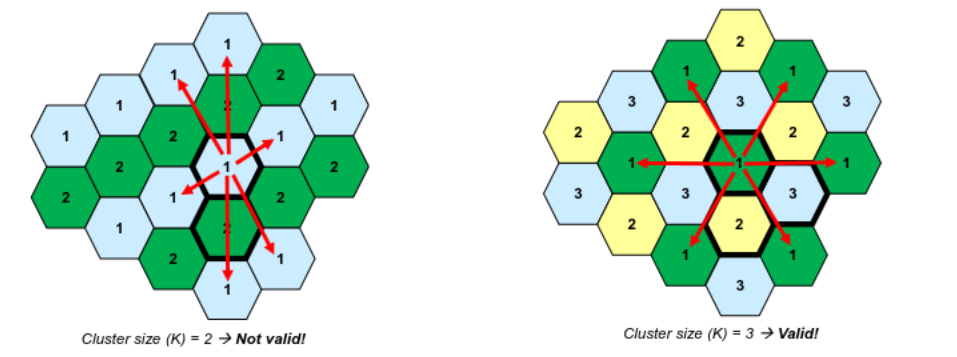
\includegraphics[width=0.8\textwidth]{pictures/8/clusterShape.png}
	\caption{Cluster shape}
\end{figure}
\subsubsection{Antenne settoriali}
L'uso di antenne settoriali, che dividono la cella in più settori, permette di ridurre le interferenze e aumentare la capacità.
Tipicamente i settori sono tre, con un angolo di 120 gradi. Il layout delle celle viene modificato, in modo che la BS non sia al centro della cella,
ma in un punto in cui i tre settori si incontrano.
\begin{figure}[H]
	\centering
	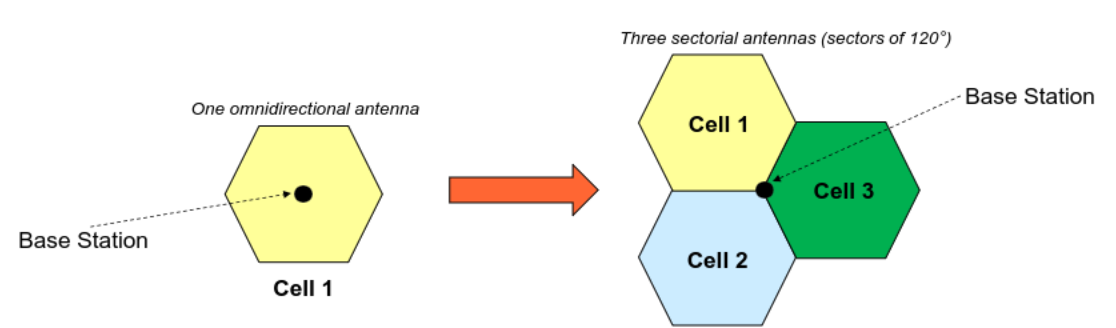
\includegraphics[width=0.8\textwidth]{pictures/8/sectorialAntennas.png}
	\caption{Sector antennas}
\end{figure}
\subsubsection{Vincoli sugli assegnamenti di frequenze}
Una volta che una dimensione di cluster $K$ è stata scelta, l'assegnamento di frequenze deve essere fatto in modo da rispettare ulteriori vincoli.
Le antenne settoriali, ad esempio, possono generare interferenza nelle celle adiacenti a causa dei side lobes, dunque le stesse frequenze non possono essere assegnate a celle/settori nello stesso punto.
\begin{figure}[H]
	\centering
	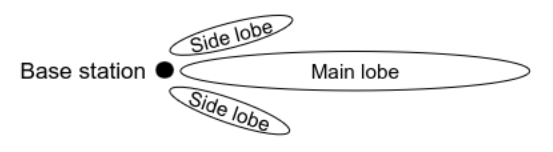
\includegraphics[width=0.6\textwidth]{pictures/8/lobe.png}
	\caption{Propagazione dei side lobes}
\end{figure}
Le frequenze adiacenti hanno spesso uno spettro di frequenze che si sovrappone leggermente, che dunque genera interferenza (interferenza di tipo adjacent channel).
Dunque, non è consigliato assegnare frequenze adiacenti a celle/settori nello stesso punto.
\subsubsection{Configurazioni multiple}
È possibile pianificare il layout delle celle in modo diverso per aree diverse, basandosi sulla densità del traffico.
Un raggio delle celle minore porta ad avere una densità per BS maggiore, di conseguenza un numero più alto di canali per unità di area e quindi più utenti possono essere serviti.
Se le celle sono già state posizionate, è possibile suddividerle in celle più piccole, con un raggio minore (cell splitting).
Questo porta a dover rieffettuare la pianificazione di copertura.
\begin{figure}[H]
	\centering
	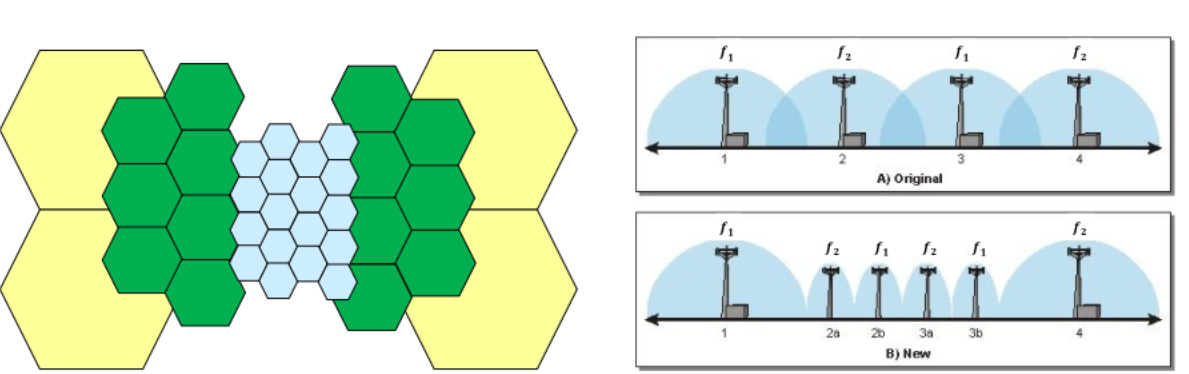
\includegraphics[width=0.8\textwidth]{pictures/8/cellSplitting.png}
	\caption{Cell splitting}
\end{figure}
Con celle più piccola, aumenta il numero di handover. La gestione della mobilità può essere semplificando creando una macro cella (ombrello) sovrapposta a quelle più piccole,
in questo modo l'UE non deve eseguire un handover quando si sposta tra le celle più piccole.
\begin{figure}[H]
	\centering
	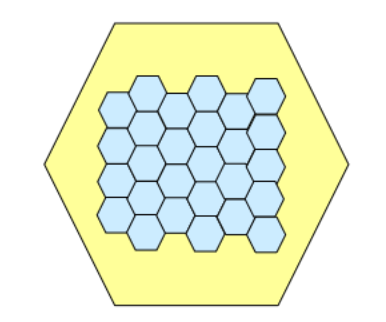
\includegraphics[width=0.3\textwidth]{pictures/8/umbrellaCell.png}
	\caption{Umbrella cell}
\end{figure}
In questo modo gli utenti a bassa mobilità vengono assegnati alle celle più piccole, mentre quelli ad alta mobilità vengono assegnati alla macro cella, riducendo il numero di handover.
